% Chapter 1
\chapter{Introducción general} % Main chapter title

Este capítulo explica los motivos detrás de la decisión de realizar este trabajo final. 
Enumera los alcances y requerimientos del trabajo, y compara al dispositivo desarrollado con productos de características similares disponibles en el mercado.

\label{Chapter1} % For referencing the chapter elsewhere, use \ref{Chapter1} 
\label{IntroGeneral}

%----------------------------------------------------------------------------------------

% Define some commands to keep the formatting separated from the content 
\newcommand{\keyword}[1]{\textbf{#1}}
\newcommand{\tabhead}[1]{\textbf{#1}}
\newcommand{\code}[1]{\texttt{#1}}
\newcommand{\file}[1]{\texttt{\bfseries#1}}
\newcommand{\option}[1]{\texttt{\itshape#1}}
\newcommand{\grados}{$^{\circ}$}

%----------------------------------------------------------------------------------------

%\section{Introducción}

%----------------------------------------------------------------------------------------
\section{Motivación}

Desde el año 1991 en adelante, todos los fabricantes de vehículos de combustión interna están obligados a incluir en sus vehículos un sistema electrónico de diagnóstico. Este sistema, conocido por sus siglas en inglés como OBD \textit{On-Board Diagnostics}, realiza las tareas de muestrear sensores que están conectados físicamente sobre el motor y alertar al conductor, a través de un indicador en el tablero, cuando el motor no está funcionando dentro de los parámetros de operación. También mantiene un registro interno de los fallos ocurridos durante la vida del mismo, para luego ser descargado por el mecánico encargado de realizar tareas de reparación o puesta a punto, y así facilitar su trabajo.
Actualmente existen grupos de entusiastas y coleccionistas que poseen vehículos fabricados antes de que el sistema OBD se haga obligatorio. Y por esa razón, no tienen la posibilidad de hacer un monitoreo del funcionamiento del motor de su vehículo. Tampoco es posible mantener un registro de si hubo eventos de fallas o momentos de operación fuera de rango, información útil para su mantenimiento preventivo.
Por esto es que se tomó la decisión de desarrollar un dispositivo que cumpla las mismas funciones que un OBD, pero para vehículos antiguos que no tienen instalado dicho sistema de fábrica.

\section{Alcance y objetivos}

El objetivo de este trabajo fue de desarrollar un prototipo que realizara las funciones de muestrear, guardar y mostrar en tiempo real, los datos adquiridos por los sensores del motor.

\subsection{Alcances}

Los alcances son:
\begin{itemize}
\item La elección de componentes electrónicos.
\item El diseño del circuito para amplificar las señales de los sensores.
\item El diseño del circuito impreso.
\item El desarrollo del firmware de la parte adquisidora.
\item El desarrollo del software de la interfaz gráfica de usuario.
\item La confección de un primer prototipo.
\item Los ensayos de verificación y validación con el prototipo.
\end{itemize}

La selección de los sensores a utilizar no formó parte los alcances porque los sensores fueron seleccionados previo al comienzo del desarrollo.

\section{Estado del arte}

Actualmente, existen en el mercado productos de características y funcionalidades similares. Para poder hacer una comparación se eligieron los productos de entrada de dos marcas distintas. Uno es el Fueltech FT-300 \citep{ft-300}, que puede verse en la figura \ref{fig:comparativa}\subref{fig:fueltech},  y el otro es el HT-193000 \citep{ht-193000} de Halltech, visto en la figura \ref{fig:comparativa}\subref{fig:halltech}. A este tipo de dispositivos se los conoce por sus siglas en inglés como ECU o \textit{Engine Control Unit}. Una ECU es un dispositivo electrónico que recopila los datos de los sensores del motor y también otros como la posición del pedal acelerador, para determinar la cantidad de combustible a inyectar y el tiempo de ignición. Además también funcionan como OBD para realizar diagnóstico y registro de fallos. Cabe destacar que al momento de escribir esta memoria, no existe un producto similar que esté diseñado o fabricado en Argentina.

\begin{figure}[htpb]
\centering
\begin{subfigure}{.4\textwidth}
\centering
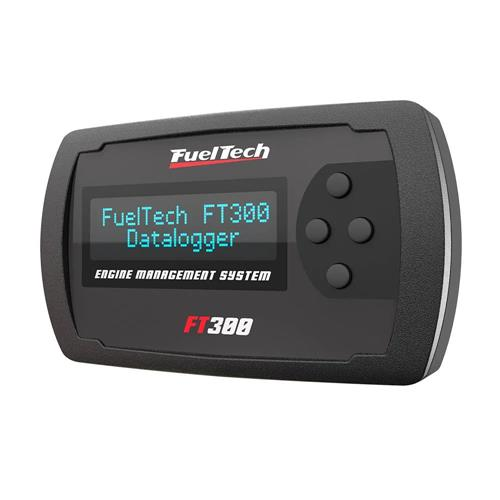
\includegraphics[width=\textwidth]{./Figures/fueltech-ft300.jpg}
\caption{Fueltech FT-300}
\label{fig:fueltech}
\end{subfigure}
\hfill
\begin{subfigure}{.5\textwidth}
\centering
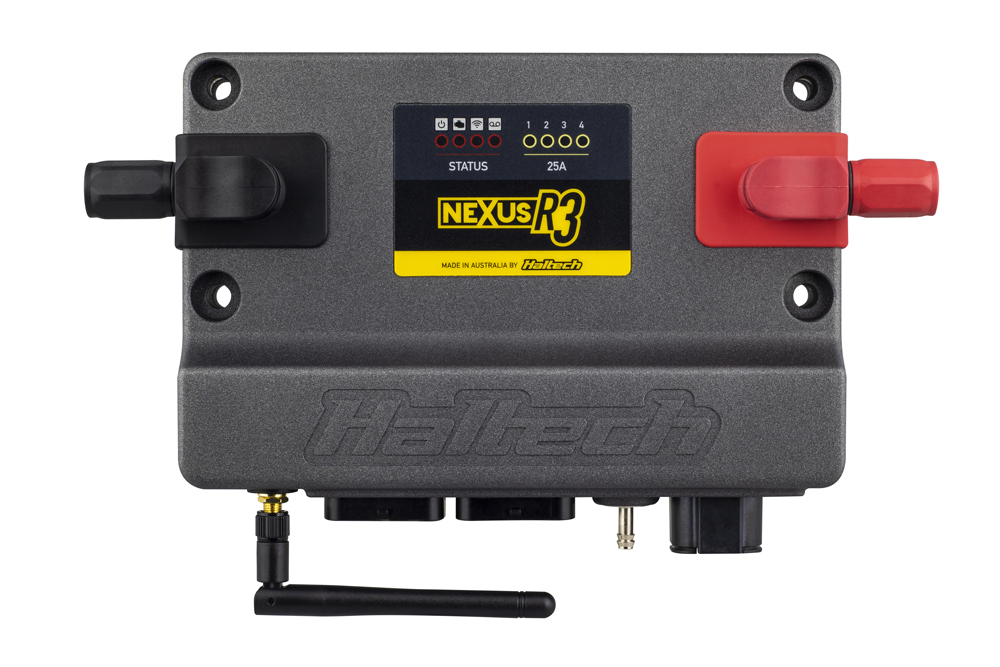
\includegraphics[width=\textwidth]{./Figures/HT-193000_00.JPG}
\caption{Halltech HT-193000}
\label{fig:halltech}
\end{subfigure}
\caption{Fotografías de ambas ECUs, a la izquierda (A) se ve la ECU FT-300 de Fueltech, y a la derecha (B) se ve la ECU HT-193000 de Halltech.\protect\footnotemark[1]}
\label{fig:comparativa}
\end{figure}
\footnotetext[1]{Imagenes tomada de \cite{ft-300} y \cite{ht-193000}}

La tabla \ref{tab:comparativa} hace una comparativa entre estos productos y el dispositivo desarrollado enlistando sus funcionalidades y características.  Como se puede ver en esa tabla, el prototipo desarrollado no posee entradas para presión de combustible, presión de admisión, y lo más importante, tampoco posee control de inyección como los otros dos productos. El hecho de que el prototipo no realice control de inyección hace que no sea clasificado como ECU y solo realiza las funciones de un sistema de diagnóstico de a bordo. Se decidió no implementar estas características para abaratar costos y no alargar el tiempo de desarrollo. Las ventajas que tiene el prototipo es que tiene una pantalla LCD para mostrar las gráficas de las evoluciones de las variables en el tiempo y puede configurarse por medio de la misma por su interfaz táctil. El FT-300 puede configurarse conectando una PC con un cable USB, el usuario configura al dispositivo usando un software que proporciona el fabricante. Y el HT-19300 se configura de la misma manera, solo que el dispositivo funciona como un punto de acceso Wi-Fi y la PC debe conectarse a la red del dispositivo para poder comunicarse.

\begin{table}[htpb]
	\centering
	\caption[Tabla comparativa entre dispositivos.]{Tabla comparativa entre dispositivos.}
	\centering
	\begin{tabular}{l c c c}    
		\toprule
		\textbf{Característica }     & \textbf{HT-193000} & \textbf{FT-300} & \textbf{Prototipo}\\
		\midrule
		Entradas de temperatura	&  0 &   2 &  3\\
		Presión de aceite		& Sí &  Sí & Sí\\
		Presión de combustible	& Sí &  Sí & No\\
		Presión de admisión		& Sí &  Sí & No\\
		Sonda Lambda			& Sí &  Sí & Sí\\
		R.P.M.					& Sí &  Sí & Sí\\
		Entradas analógicas		& 11 &  0  &  0\\
		Control de inyección	& Sí &  Sí & No\\
		Interfaz gráfica		& No &  Matriz de puntos & Pantalla LCD \\
		Configuración			& Wi-Fi & USB & Interfaz táctil \\ 
		\bottomrule
	\end{tabular}
	\label{tab:comparativa}
\end{table}